\section{\textbf{\underline{ANEXO 2: Resultados simulación}}}
La simulación realizada en el software de INCONTROL \textit{Enterprise Dynamics} se ha realizado sobre todo el sistema, durrante 24 horas y con 150 réplicas. A continuación se adjuntan los resultados obtenidos:

\begin{figure}[H]
\begin{center}
\centering
  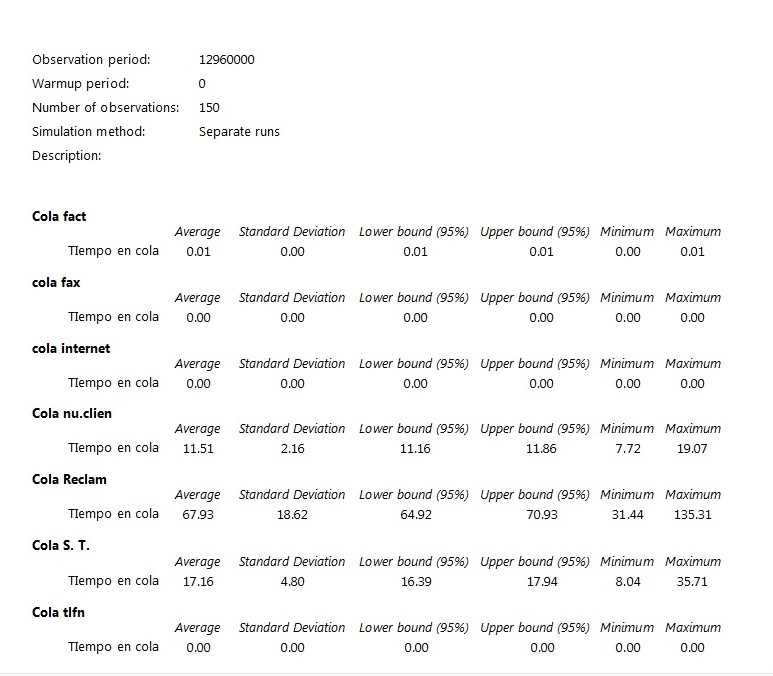
\includegraphics[width=1\textwidth]{./images/foto1}
  \caption{Resultados de la simulación 1}
  \label{fig: Resultados de la simulacion 1}
\end{center}
\end{figure}
\begin{figure}[H]
\begin{center}
\centering
  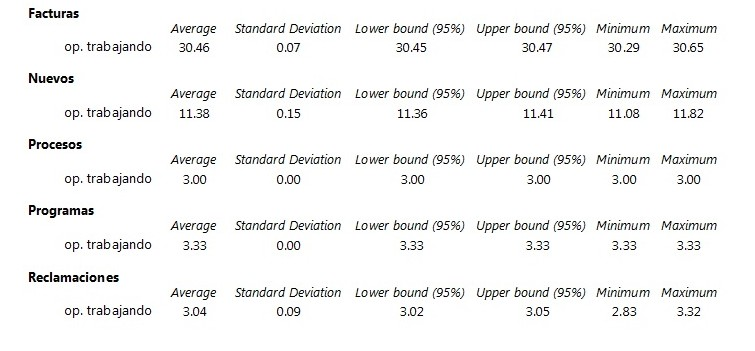
\includegraphics[width=1\textwidth]{./images/foto2}
  \caption{Resultados de la simulación 2}
  \label{fig: Resultados de la simulacion 2}
\end{center}
\end{figure}
\begin{figure}[H]
\begin{center}
\centering
  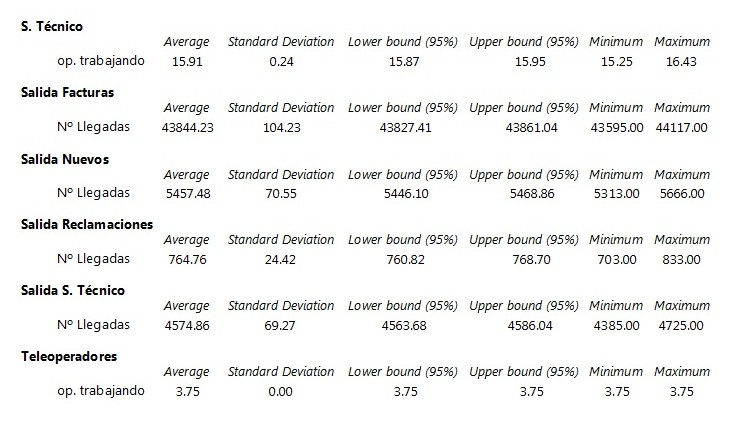
\includegraphics[width=1\textwidth]{./images/foto3}
  \caption{Resultados de la simulación 3}
  \label{fig: Resultados de la simulacion 3}
\end{center}
\end{figure}
Por tanto, podemos obtener directamente el tiempo medio de espera en cada cola, así como el tráfico pasa por cada servidor. Para calcular la saturación del servidor basta con obtener el cociente entre el número medio de servidores activos obtenidos en la simulación ($X_{i}$) y el número de operarios totales para cada servidor $i$ ($op.s_{i}$):
\begin{multline}\\
p_{1 simulado} = \frac{X_{1}}{op.s_{1}} = \frac{3,75}{5} = 0,75 \\
p_{2 simulado} = \frac{X_{2}}{op.s_{2}} = \frac{3,33}{4} = 0,832\\
p_{3 simulado} = \frac{X_{3}}{op.s_{3}} = \frac{3}{4} = 0,75\\
p_{4 simulado} = \frac{X_{4}}{op.s_{4}} = \frac{30,46}{36} = 0,846\\
p_{5 simulado} = \frac{X_{5}}{op.s_{5}} = \frac{11,38}{14} = 0,813\\
p_{6 simulado} = \frac{X_{6}}{op.s_{6}} = \frac{3,04}{4} = 0,76\\
p_{7 simulado} = \frac{X_{7}}{op.s_{7}} = \frac{15,91}{19} = 0,837\\
\end{multline}
